\documentclass{beamer}
\usepackage{amsmath,amsbsy,amsopn,amstext,amsfonts,amssymb}
\usepackage{isomath}
\usepackage{ulem}
%\linespread{1.6}  % double spaces lines
\usepackage{graphicx}
\usepackage{subfigure}
\usepackage{color}
\usepackage{optidef}  % define optimization problems
\usepackage{multicol}  % multiple columns
\usepackage{listings} % for python code
\usepackage{mathrsfs}

\usepackage{polynom}
\newcommand{\adj}{\mathrm{adj}}
\newcommand{\constrainedmin}[3]{
		\begin{mini*}|s|
		{#2}{#1}{}{}
		\addConstraint{#3}
		\end{mini*}
}

\newcommand{\rwbcomment}[1]{{\color{blue}RWB:#1}}
\newcommand{\defeq}{\stackrel{\triangle}{=}}
\newcommand{\abs}[1]{\left|#1\right|}
\newcommand{\norm}[1]{\left\|#1\right\|}
\newcommand{\iprod}[1]{\left<#1\right>}
\newcommand{\ellbf}{\boldsymbol{\ell}}
\newcommand{\nubf}{\boldsymbol{\nu}}
\newcommand{\mubf}{\boldsymbol{\mu}}
\newcommand{\abf}{\mathbf{a}}
\newcommand{\bbf}{\mathbf{b}}
\newcommand{\cbf}{\mathbf{c}}
\newcommand{\dbf}{\mathbf{d}}
\newcommand{\ebf}{\mathbf{e}}
\newcommand{\fbf}{\mathbf{f}}
\newcommand{\gbf}{\mathbf{g}}
\newcommand{\hbf}{\mathbf{h}}
\newcommand{\ibf}{\mathbf{i}}
\newcommand{\jbf}{\mathbf{j}}
\newcommand{\kbf}{\mathbf{k}}
\newcommand{\lbf}{\mathbf{l}}
\newcommand{\mbf}{\mathbf{m}}
\newcommand{\nbf}{\mathbf{n}}
\newcommand{\obf}{\mathbf{o}}
\newcommand{\pbf}{\mathbf{p}}
\newcommand{\qbf}{\mathbf{q}}
\newcommand{\rbf}{\mathbf{r}}
\newcommand{\sbf}{\mathbf{s}}
\newcommand{\tbf}{\mathbf{t}}
\newcommand{\ubf}{\mathbf{u}}
\newcommand{\vbf}{\mathbf{v}}
\newcommand{\wbf}{\mathbf{w}}
\newcommand{\xbf}{\mathbf{x}}
\newcommand{\ybf}{\mathbf{y}}
\newcommand{\zbf}{\mathbf{z}}
\newcommand{\Jbf}{\mathbf{J}}
\newcommand{\Acal}{\mathcal{A}}
\newcommand{\Bcal}{\mathcal{B}}
\newcommand{\Lcal}{\mathcal{L}}
\newcommand{\Ncal}{\mathcal{N}}
\newcommand{\Rcal}{\mathcal{R}}
\definecolor{darkolivegreen}{rgb}{0.33, 0.42, 0.18}

\makeatletter
\newenvironment<>{proofstart}[1][\proofname]{%
    \par
    \def\insertproofname{#1\@addpunct{.}}%
    \usebeamertemplate{proof begin}#2}
  {\usebeamertemplate{proof end}}
\newenvironment<>{proofcont}{%
  \setbeamertemplate{proof begin}{\begin{block}{}}
    \par
    \usebeamertemplate{proof begin}}
  {\usebeamertemplate{proof end}}
\newenvironment<>{proofend}{%
    \par
    \pushQED{\qed}
    \setbeamertemplate{proof begin}{\begin{block}{}}
    \usebeamertemplate{proof begin}}
  {\popQED\usebeamertemplate{proof end}}
\makeatother

\title{ECEn 671: Mathematics of Signals and Systems}
\author{Randal W. Beard}
\institute{Brigham Young University}
\date{\today}

\begin{document}

%-------------------------------
\begin{frame}
	\titlepage
\end{frame}



%%%%%%%%%%%%%%%%%%%%%%%%%%%%%%%%%%%%%%%%%%%%%%%%%%%%%%%%%%%%%%%%%
\section{Equality Constraints: Lagrange Multipliers}
\frame{\sectionpage}

%----------------------------------
\begin{frame}\frametitle{Equality Constraints: Lagrange Multipliers}
	Several geometric insights help:
	
	{\color{blue}Insight  \#1} 
	\begin{itemize}
		\item Geometrically what do the constraints $\hbf(x) = 0$ look like?
		\item What if $\hbf$ is linear, i.e. $\hbf(x) = Hx = 0$ where $H:\mathbb{R}^n\to\mathbb{R}^m$.
		\item The constraint implies that $x$ must be in the null space of $H$, which is a linear space of dimension $n-m$, i.e. an $n-m$ dimensional hyperplane.
		\item In general, $\hbf(x)=0$ is an $n-m$ dimensional hypersurface in $\mathbb{R}^n$.
	\end{itemize}

	\begin{center}
		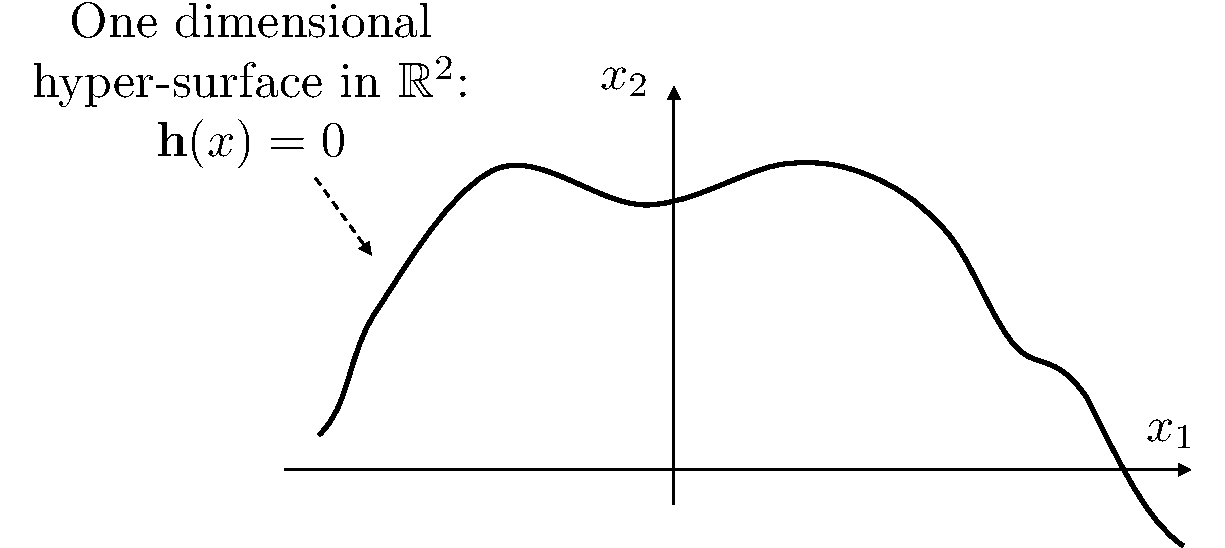
\includegraphics[width=0.5\textwidth]
			{figures/chap18_hypersurface}
	\end{center}
	
\end{frame}

%----------------------------------
\begin{frame}\frametitle{Equality Constraints: Lagrange Multipliers}
	{\color{blue}Insight  \#2}
	\begin{center}
		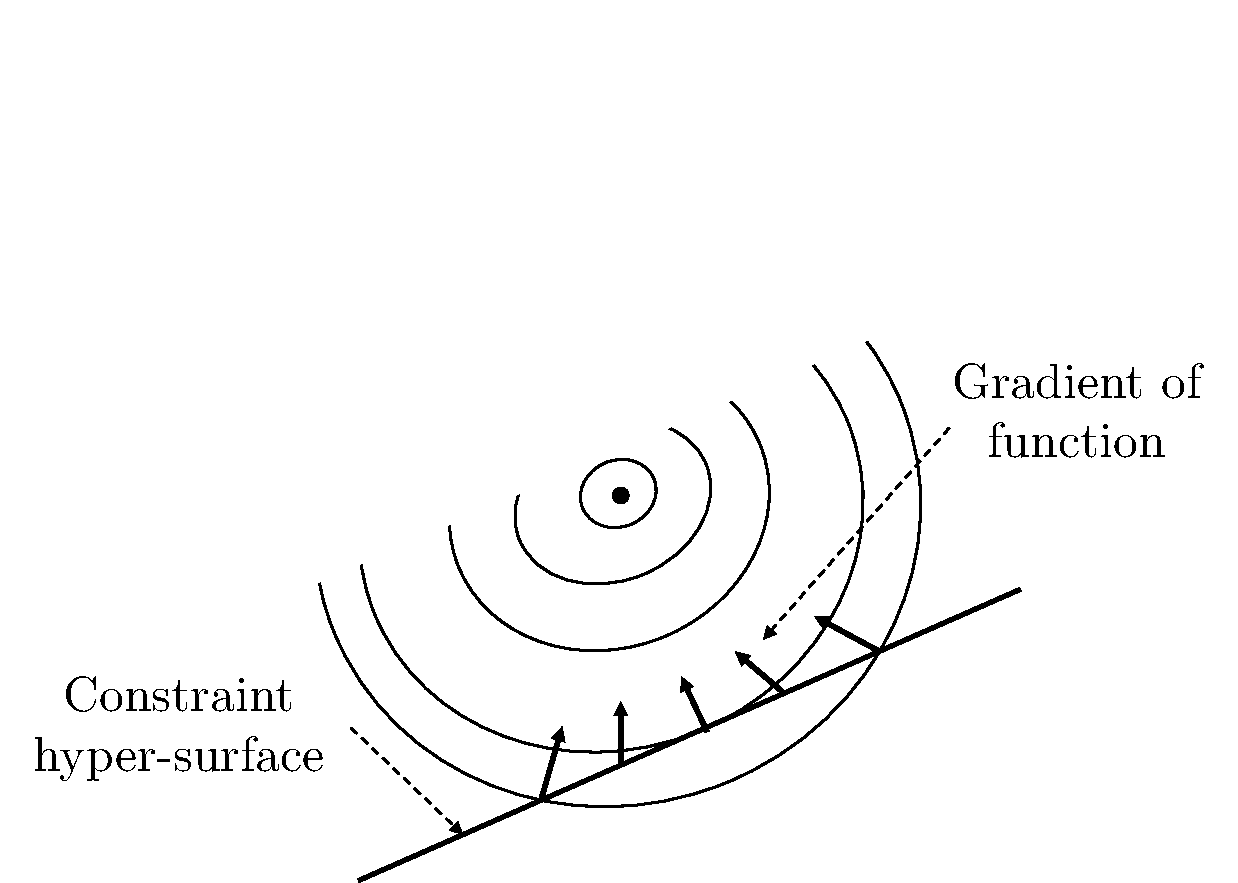
\includegraphics[width=0.5\textwidth]
			{figures/chap18_gradient_on_constraint}
	\end{center}
	
	At a constrained minimum the gradient is orthogonal to the hypersurface.
\end{frame}

%----------------------------------
\begin{frame}\frametitle{Equality Constraints: Lagrange Multipliers}
	To formalize, we need some definitions.
	
	Let $\mathbb{S}$ be a hyper-surface of dimension $n-m$.  Let $x$ be a curve on $\mathbb{S}$ continuously parameterized by $\xi \in [a,b]$, i.e. $x(\xi) \in \mathbb{S}$.
	
	\begin{center}
		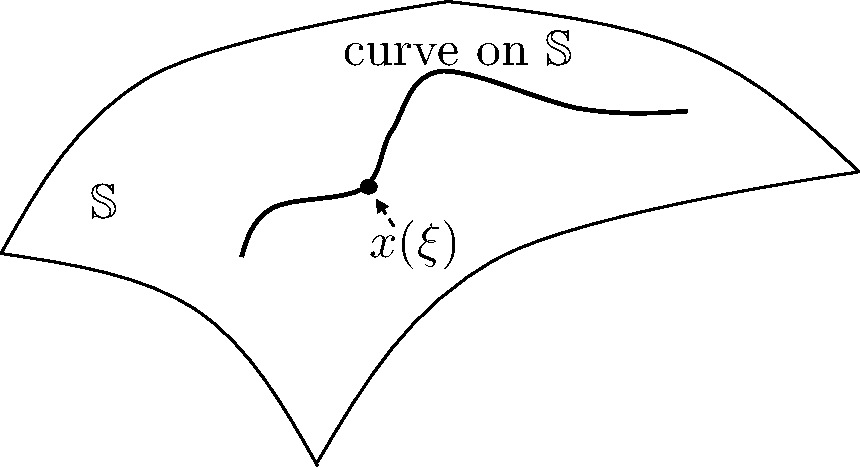
\includegraphics[width=0.5\textwidth]
			{figures/chap18_curve_on_S}
	\end{center}
	
	The derivative of the curve at $x(\xi_0)$ is 
	\[
		\dot{x}(\xi_0) = \frac{d}{d\xi}x(\xi_0).
	\]	
\end{frame}

%----------------------------------
\begin{frame}\frametitle{Equality Constraints: Lagrange Multipliers}
	\begin{definition}
		The \underline{tangent plane} to a surface $\mathbb{S}$ at $x \in \mathbb{S}$ is the span of the derivatives of all the differentiable curves on $\mathbb{S}$ at $x$.
	\end{definition}
	
	\vfill

	The problem with this definition is that it is not constructive, i.e. it doesn't give us a good way to actually construct the tangent plane.
	
\end{frame}

%----------------------------------
\begin{frame}\frametitle{Equality Constraints: Lagrange Multipliers}
	To construct the tangent plane, recall that the gradient of $\hbf(x)$ is orthogonal to level curves of $\hbf(x)$:
	\begin{center}
		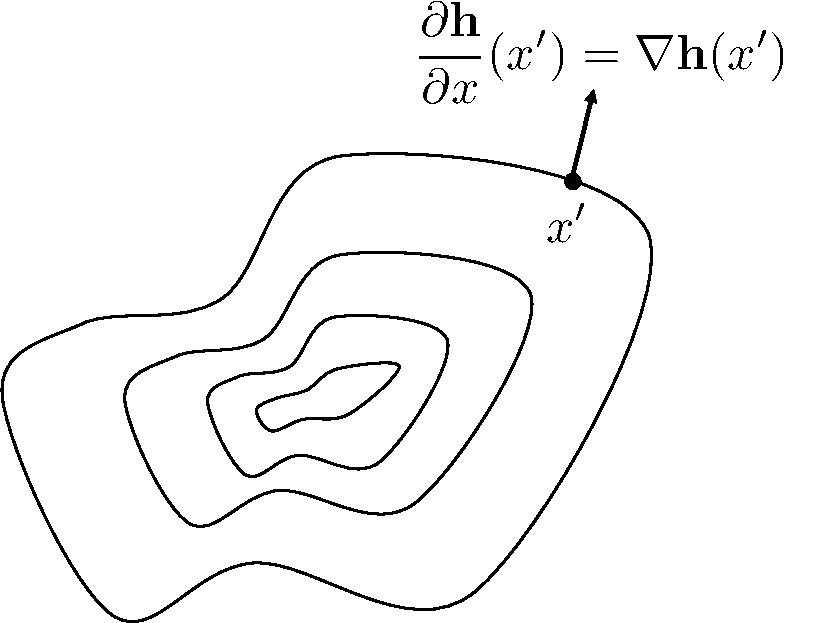
\includegraphics[width=0.3\textwidth]
			{figures/chap18_gradient_h}
	\end{center}	
	Also recall that the formula for the plane is
	\[
		\left\{ y\in \mathbb{R}^n \mid \nbf^\top (y-x^{\ast})=0 \right\}.
	\]
	\begin{center}
		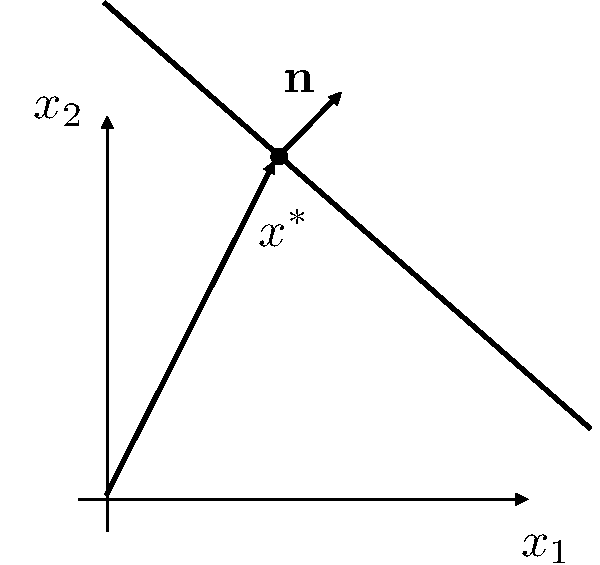
\includegraphics[width=0.3\textwidth]
			{figures/chap18_line}
	\end{center}
\end{frame}

%----------------------------------
\begin{frame}\frametitle{Equality Constraints: Lagrange Multipliers}
	Therefore the tangent plane of $h(x)$ at $x^{\ast}$ is given by
	\[ 
		P = \{ y\in \mathbb{R}^n \mid \nabla \hbf^\top (x^{\ast})(y-x^{\ast}) =0 \} 
	\]
	where $\nabla \hbf^\top (x^{\ast})$ defines an $n-m$ dimensional plane if the rows are linearly independent.

	\begin{definition}
		When the gradient vectors $\nabla h_1, \nabla h_2, \ldots, \nabla h_m$ are linearly independent at $x^{\ast}$, $x^{\ast}$ is called a \underline{regular point}.	 
	\end{definition}

	\vfill
	
	We will always assume ``regularity'' of the constraints.
\end{frame}
	
%----------------------------------
\begin{frame}\frametitle{Equality Constraints: Lagrange Multipliers}
	\begin{lemma}[Moon Lemma 18.1]
		Let $x(\xi)$ be a curve on $\hbf(x) = 0$ such that 
		\[
			\left. x(\xi)\right|_{\xi=0} = x^{\ast},
		\] 
		is a constrained local minimum of $f$.		
		Then 
		\[
			\left. \displaystyle\frac{d}{d\xi}f(x(\xi))\right|_{\xi=0} = 0.
		\]		
	\end{lemma}
	Geometry: at point $p$, $f$ is neither increasing nor decreasing along $x(\xi)$.
	\begin{center}
		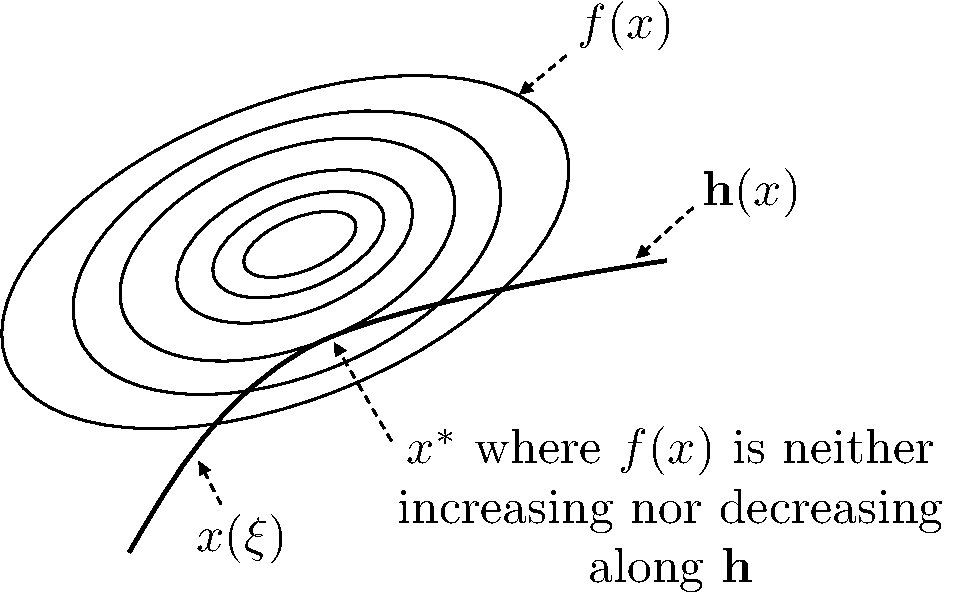
\includegraphics[width=0.4\textwidth]
			{figures/chap18_constraint_along_h}
	\end{center}
		
\end{frame}

%----------------------------------
\begin{frame}\frametitle{Equality Constraints: Lagrange Multipliers: Proof}
	\begin{proof}
		Expanding $f(x(\xi))$ in a Taylor series:
		\[ 
			f(x(\xi)) = \left. f(x(0)) + \xi\frac{d}{d\xi}f(x(\xi))\right|_{\xi=0} + O(|\xi|) 
		\]
		If $f(x(0))$ is a local minimum then for $\abs{\xi}$-small
		\[ 
			\left. \xi\frac{d}{d\xi}f(x(\xi))\right|_{\xi =0} \geq 0 
		\]
		for all $\xi$ both positive and negative.  Therefore
		\[ 
			\left. \frac{d}{df}f(x(\xi))\right|_{\xi=0} = 0 
		\]
		where
		\( 
			\frac{d}{d\xi}f(x(\xi)) = \nabla^\top f(x(\xi)) \dot{x}(\xi)
		\)
		and $\dot{x}(\xi)$ is an element of the tangent plane.
	\end{proof}
\end{frame}

%----------------------------------
\begin{frame}\frametitle{Equality Constraints: Lagrange Multipliers}
	\begin{lemma}[Moon Lemma 18.2]
		If $x^{\ast}$ is a regular point of $\hbf(x) = 0$ \underline{and} a local constrained minimum, then 
		\[ 
			\nabla \hbf^\top (x^{\ast})y = 0 \Rightarrow \nabla f^\top (x^{\ast})y = 0 
		\]
		i.e. if $y$ is in the tangent plane of $\hbf$ at $x^{\ast}$, then $y$ is orthogonal to the gradient of $f$.	
	\end{lemma}
	\begin{center}
		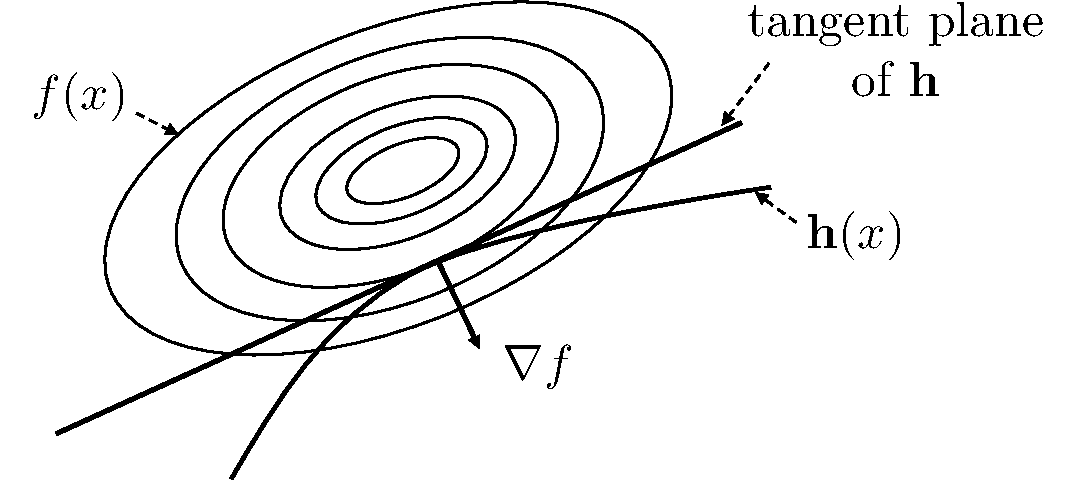
\includegraphics[width=0.5\textwidth]
			{figures/chap18_tangent_plane_of_h}
	\end{center}	
\end{frame}

%----------------------------------
\begin{frame}\frametitle{Proof of Lemma 18.2}
	\begin{proof}
		Translate the coordinate system such that $x^{\ast} = 0$.  Regularity implies that the tangent plane is given by 
		\[ 
			P(x^{\ast}) \defeq \{ z\in \mathbb{R}^n \mid \nabla \hbf^\top (x^{\ast})z = 0 \} 
		\]
		Let $y \in P(x^{\ast})$ then 
		\[
			\nabla \hbf^\top (x^{\ast}) y = 0.
		\]
		
		\vfill
		
		Now choose a smooth curve $x(\xi)$ on $\hbf(x) = 0$ such that $x(0) = x^{\ast}$ and $\dot{x}(0) = y$.
		
		\vfill
		
		From Lemma 18.1, $\nabla f^\top (x^{\ast})y = 0$. 
	\end{proof}
\end{frame}

%----------------------------------
\begin{frame}\frametitle{Key Insight}
	At a constrained local minimum $\nabla f(x^{\ast})$ and the columns of $\nabla \hbf(x^{\ast})$ are parallel, i.e., there is some scalar $\mu_i$ such that
	\begin{align*}
		& \nabla f(x^{\ast}) = \mu_i\nabla h_i(x^{\ast}) \qquad i= 1,\ldots,m \\
		\implies & m\nabla f(x^{\ast}) = \sum_{i=1}^m \mu_i \nabla h_i (x^{\ast}) \\
		\implies & \nabla f(x^{\ast}) - \sum_{i=1}^m \frac{\mu_i}{m}\nabla h_i(x^{\ast}) = 0\\
		\implies & \fbox{$\nabla f(x^{\ast}) + \nabla \hbf(x^{\ast}) \lambda = 0$}
	\end{align*}
	where 
	\[
		\lambda = \begin{pmatrix}
	    			-\frac{\mu_1}{m} &
	    			\dots &
	    			-\frac{\mu_m}{m}
	  			  \end{pmatrix}^\top.
	\]
	The vector $\lambda \in \mathbb{R}^m$ is called the \underline{Lagrange Multiplier}.	
\end{frame}

%----------------------------------
\begin{frame}\frametitle{Necessary Conditions}
	\begin{theorem}[Moon Theorem 18.3 (Necessary conditions for equality constraints)]
		Let $x^{\ast}$ be a local extremum of $f$ subject to the constraints $h(x) = 0$, and let $x^{\ast}$ be a regular point.  Then there is a $\lambda \in \mathbb{R}^n$ such that
		\[ 
			\nabla f(x^{\ast}) + \nabla \hbf(x^{\ast})\lambda = 0.
		\]
	\end{theorem}	
	\begin{corollary}
		Let 
		\[ 
			L(x,\lambda) = f(x) + \hbf^\top(x)\lambda.
		\]
		Then if $x^{\ast}$ is a regular local extremum, then
		\[ 
			\nabla_x L(x^{\ast},\lambda^{\ast}) = \frac{\partial L}{\partial x}(x^{\ast},\lambda^{\ast}) = 0 
		\]
		and
		\[ 
			\nabla_{\lambda}L(x^{\ast},\lambda^{\ast}) = \frac{\partial L}{\partial \lambda}(x^{\ast},\lambda^{\ast}) = 0.
		\]
	\end{corollary}
\end{frame}
	
%----------------------------------
\begin{frame}\frametitle{Proof of Theorem 18.3}
	\begin{proof}
		\begin{eqnarray}
		\label{eqn18.3.1} \frac{\partial L}{\partial x} = \nabla f(x^{\ast}) + \nabla h(x^{\ast}) \lambda^{\ast} = 0 \\
		\label{eqn18.3.2} \frac{\partial L}{\partial \lambda} = h(x^{\ast}) = 0
		\end{eqnarray}
		Equation (\ref{eqn18.3.2}) implies that the constraints are satisfied.
		
		Equation (\ref{eqn18.3.1}) comes from Theorem 18.3.
	\end{proof}
\end{frame}

%----------------------------------
\begin{frame}\frametitle{Lagrange Multipliers: Example 1}
	\begin{mini*}|s|
		{}{x_1^2 + x_2^2}{}{}
		\addConstraint{x_1 + x_2 = 2}
	\end{mini*}
	\begin{center}
		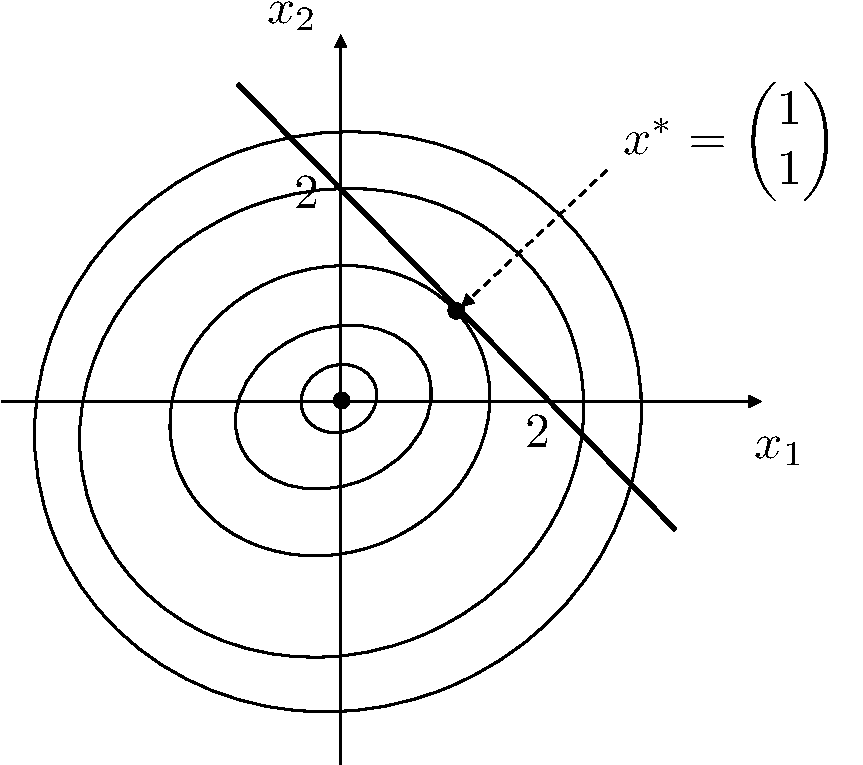
\includegraphics[width=0.5\textwidth]
			{figures/chap18_example1}
	\end{center}
	The Lagrangian is
	\[ 
		L = x_1^2 + x_2^2 + \lambda(x_1 + x_2 - 2). 
	\]	
\end{frame}
	
%----------------------------------
\begin{frame}\frametitle{Lagrange Multipliers: Example 1, cont.}
	The necessary conditions for a minimum are
	\begin{align*}
		\frac{\partial L}{\partial x_1} &= 2x_1 + \lambda = 0 \quad \implies x_1 = -\frac{\lambda}{2}\\
		\frac{\partial L}{\partial x_2} &= 2x_2 + \lambda = 0 \quad \implies x_2 = -\frac{\lambda}{2}\\
		\frac{\partial L}{\partial \lambda} &= x_1 + x_2 - 2 = 0 \quad \implies -\lambda - 2 = 0.
	\end{align*}
	Therefore $\lambda = -2$, $x_1 = 1$, $x_2 = 1$, which implies that 
	\[
			x^{\ast} 
				= 
				\begin{pmatrix}
	      			1 \\ 1
	    		\end{pmatrix}
	\]
	as expected.	
\end{frame}

%----------------------------------
\begin{frame}\frametitle{Lagrange Multipliers: Example 18.4.7 (Maximum Entropy)}
	Let $\mathbb{X}$ be a random variable with probability mass function $p(\mathbb{X}=x_i) = p_i \qquad i = 1, \ldots, m$,
	
	Then, the entropy of $\mathbb{X}$ is defined as
	\[ 
		H = -\sum_{i=1}^m p_i\log p_i 
	\]	
	Question:  Which pmf has maximum entropy?
	
	\vfill
	
	To answer, lets solve the optimization problem:
	\begin{maxi*}|s|
		{}{H}{}{}
		\addConstraint{\sum p_i = 1}
		\addConstraint{p_i \geq 0}
	\end{maxi*}
\end{frame}

%----------------------------------
\begin{frame}\frametitle{Lagrange Multipliers: Example 18.4.7 (Maximum Entropy)}
	Lets ignore the inequality constraint for now and go back later.
	
	The Lagrangian is
	\[ 
		L = -\sum p_i \log p_i + \lambda(\sum p_i - 1) 
	\]
	The necessary conditions are
	\begin{align*}
		\frac{\partial L}{\partial p_i} &= 0 \qquad i = 1, \ldots, m\\
		\frac{\partial L}{\partial \lambda} &= 0
	\end{align*}
	where
	\begin{align*}
		& \frac{\partial L}{\partial p_i} = -\log p_i - 1 + \lambda = 0 \qquad i = 1, \ldots, m\\
		\implies & \lambda = 1+\log p_i\\
		\implies & \log p_i = \lambda - 1.
	\end{align*}	
\end{frame}

%----------------------------------
\begin{frame}\frametitle{Lagrange Multipliers: Example 18.4.7 (Maximum Entropy)}
	So $p_i$ must be constant for all $i$.  The constant $\sum p_i = 1 \Rightarrow p_i = \frac{1}{n} \geq 0$, so $p_i$ satisfies the inequality constraint.
	
	\vfill
	
	In other words: the uniform pmf maximizes entropy.
	
	\vfill
	
	In other words: all possibilities are equally likely.	
\end{frame}

%----------------------------------
\begin{frame}\frametitle{Lagrange Multipliers: Example: Constrained Least Squares}
	Given an ellipsoid and a point $y$ outside the ellipsoid, find the point $z$ in the ellipsoid nearest to $y$.\\
	\begin{center}
		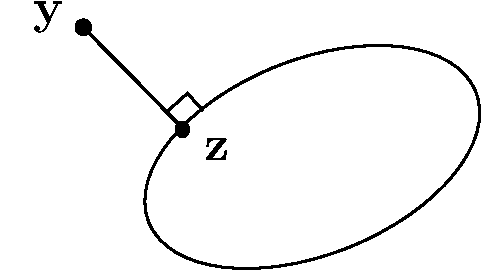
\includegraphics[width=0.5\textwidth]
			{figures/chap18_closest_point_to_set}
	\end{center}
	The equation for an ellipsoid is given by
	\[ 
		E = \{ z\in \mathbb{R}^n : z^\top L^\top Lz \leq 1.
	\]	
\end{frame}

%----------------------------------
\begin{frame}\frametitle{Lagrange Multipliers: Example: Constrained Least Squares}
	So we need to solve the following constrained optimization problem:
	\begin{mini*}|s|
		{z\in\mathbb{R}^n}{\norm{z-y }}{}{}
		\addConstraint{z^\top L^\top Lz = 1}
	\end{mini*}
	The Lagrangian is
	\[ 
		L = (y - z)^\top (y - z) + \lambda(z^\top L^\top Lz - 1) 
	\]
	
\end{frame}

%----------------------------------
\begin{frame}\frametitle{Lagrange Multipliers: Example: Constrained Least Squares}
	The necessary conditions are
	\begin{align*}
		\frac{\partial L}{\partial z} &= -2(y - z) + 2\lambda L^\top Lz = 0 \\
		\frac{\partial L}{\partial \lambda} &= z^\top L^\top Lz - 1 = 0
	\end{align*}
	The first equations gives
	\begin{align*}
		& (I + \lambda L^\top L)z = y \\
		\implies & z = (I + \lambda L^\top L)^{-1}y.
	\end{align*}
	Therefore, $\lambda$ must satisfy
	\[ 
		g(\lambda) = y^\top (I+\lambda L^\top L)^{-1}L^\top L(I + \lambda L^\top L)^{-1}y = 1 
	\]
	which must be solved numerically using a  root finding technique using e.g. Newton's method.	
\end{frame}

%----------------------------------
\begin{frame}\frametitle{Lagrange Multipliers: Example}
	Consider the following optimization problem:
	\begin{mini*}|s|
		{x\in\mathbb{R}^n}{\frac{1}{2}x^\top Ax}{}{}
		\addConstraint{Bx = c}
	\end{mini*}		
	where $A\in\mathbb{R}^{n\times n}$, 
	$B\in\mathbb{R}^{m\times n}$, 
	$c \in \mathbb{R}^{m}$.
	
	The Lagrangian is
	\[ 
		L = \frac{1}{2}x^\top Ax + \lambda^\top (Bx - c) 
	\]
\end{frame}

%----------------------------------
\begin{frame}\frametitle{Lagrange Multipliers: Example}
	The necessary conditions are
	\begin{align*}
		\frac{\partial L}{\partial x} &= Ax + B^\top \lambda = 0 \\
		\frac{\partial L}{\partial \lambda} &= Bx - c = 0
	\end{align*}
	If $A$ is invertible, then
	\begin{align*}
		& x = -A^{-1}B^\top \lambda	\\
		\implies & -BA^{-1}B^\top \lambda = c.
	\end{align*}
	If $BA^{-1}B^\top$ is invertible then
	\begin{align*}
		& 	\lambda = -(BA^{-1}B^\top )^{-1}c \\
		\implies & x = A^{-1}B^\top (BA^{-1}B^\top )^{-1}c
	\end{align*}
	which is the weighted norm pseudo-inverse.	
\end{frame}

%%%%%%%%%%%%%%%%%%%%%%%%%%%%%%%%%%%%%%%%%%%%%%%%%%%%%%%%%%%%%%%%%
\section{Sufficient Conditions}
\frame{\sectionpage}

%----------------------------------
\begin{frame}\frametitle{Lagrange Multipliers: Sufficient Conditions}
	The necessary conditions tell us where a local extremum might exist, but not whether it is a local min, max, or saddle point.
	
	\vfill
	
	Are there sufficient conditions for constrained optimization problems?	
\end{frame}

%----------------------------------
\begin{frame}\frametitle{Lagrange Multipliers: Sufficient Conditions}
	For the unconstrained problem, we look at the Hessian of $f$ for sufficient conditions.  For unconstrained problems we look at the second derivative of $L$ with respect to $x$.
	
	\vfill
	
	\[ 
		\underbrace{L}_{1\times 1} = \underbrace{f}_{1\times 1} + \underbrace{\lambda^\top }_{1\times m}\underbrace{h}_{m\times 1} = f + \sum_{i=1}^m\lambda_i h_i 
	\]
	so
	\[ 
		\underbrace{\nabla_x L}_{n\times 1} = \underbrace{\nabla_xf}_{n\times 1} + \underbrace{\nabla h}_{n\times m}\underbrace{\lambda}_{m\times 1} = \nabla_xf + \sum_{i=1}^m\lambda_i\nabla_x h_i 
	\]
	\[ 
		\nabla_{xx}^2L = \nabla_{xx}^2f + \sum_{i=1}^m\lambda_i\nabla_{xx}^2 h_i  
	\]
	We will drop the $xx$ notation (unless not obvious) to get
	
	\[ 
		\fbox{$\nabla^2L = \nabla^2f + \displaystyle\sum_{i=1}^m\lambda_i\nabla^2h_i$}
	\]	
\end{frame}

%----------------------------------
\begin{frame}\frametitle{Lagrange Multipliers: Sufficient Conditions}
	Let $P(x^{\ast}) = \{ y\in \mathbb{R}^n \mid \nabla h(x^{\ast})y = 0 \}$ be the tangent plane at $x^{\ast}$.

	\begin{theorem}[Moon Theorem 18.4]
		Let $f$ and $h$ be $C^2$
		
		1. (Necessity) Suppose that $x^{\ast}$ is a local constrained min of $f$ and that $x^{\ast}$ is regular.  Then $\exists \lambda$ such that
		\[ 
			\nabla f(x^{\ast}) + \nabla h(x^{\ast})\lambda = 0. 
		\]
		
		2. (Sufficiency)  If 
		\begin{enumerate}
		  \item $h(x^{\ast})$ = 0
		  \item $\exists \lambda$ such that $\nabla f(x^{\ast}) + \nabla h(x^{\ast}) \lambda = 0$ 
		  \item $y^\top \nabla^2L(x^{\ast})y \geq 0 \qquad \forall y\in P(x^{\ast})$
		\end{enumerate}
		 then $x^{\ast}$ is a local constrained min of $f$. 		
	\end{theorem}
\end{frame}

%----------------------------------
\begin{frame}\frametitle{Lagrange Multipliers: Sufficient Conditions: Example 18.5.1}
	\begin{maxi*}|s|
		{}{x_1x_2 + x_2x_3 + x_1x_3}{}{}
		\addConstraint{x_1 + x_2 + x_3 = 3}
	\end{maxi*}
	The Lagrangian is
	\[ 
		L = x_1x_2 + x_2x_3 + x_1x_3 + \lambda(x_1 + x_2 + x_3 - 3) 
	\]
	The necessary conditions are therefore
	\begin{align*}
		\nabla_x L  
			&= \begin{pmatrix}
	    		x_2 + x_3 + \lambda\\
	    		x_1 + x_3 + \lambda \\
	    		x_2 + x_1 + \lambda
	  		 \end{pmatrix} 
	  	 = \begin{pmatrix}
	    		0\\0\\0
	  	   \end{pmatrix} \\
		\nabla_\lambda L &= x_1 + x_2 + x_3 - 3 = 0 
	\end{align*}
\end{frame}

%----------------------------------
\begin{frame}\frametitle{Lagrange Multipliers: Sufficient Conditions: Example 18.5.1}
	Therefore, we must solve
	\[ 
		\begin{pmatrix}
	    	0 & 1 & 1 & 1\\
	    	1 & 0 & 1 & 1\\
	    	1 & 1 & 0 & 1\\
	    	1 & 1 & 1 & 0
	  	\end{pmatrix}
	  	\begin{pmatrix}
	    	x_1\\
	    	x_2\\
	    	x_3\\
	    	\lambda
	  	\end{pmatrix} 
	  	= \begin{pmatrix}
	    	0\\0\\0\\3
	  	  \end{pmatrix}.
	\]
	The solution is:
	\[ 
		\begin{pmatrix}
	    	x_1\\
	    	x_2\\
	    	x_3\\
	    	\lambda 
	  	\end{pmatrix}^\ast
	  	= \begin{pmatrix}
	    	1\\1\\1\\-2
	  	  \end{pmatrix}
	\]
\end{frame}

%----------------------------------
\begin{frame}\frametitle{Lagrange Multipliers: Sufficient Conditions: Example 18.5.1}
	Is the soluution a local max?
	
	\[ 
		\nabla^2L 
			= \begin{pmatrix}
	    		0 & 1 & 1\\
	    		1 & 0 & 1\\
	    		1 & 1 & 0
	  		  \end{pmatrix} 
	  		  + \lambda \begin{pmatrix}
	    					0 & 0 & 0\\
	    					0 & 0 & 0\\
	    					0 & 0 & 0
	  					\end{pmatrix}
	\]
	Note that 
	\[
		\text{eig}
			\begin{pmatrix}
	    		0 & 1 & 1\\
	    		1 & 0 & 1\\
	    		1 & 1 & 0   
	  		\end{pmatrix} = -1, -1, 2 
	\]
	and so $\nabla^2L$ is indefinite.  
	
	\vfill
	
	However, the sufficient condition requires that we restrict attention to $P(x^{\ast})$.
\end{frame}

%----------------------------------
\begin{frame}\frametitle{Lagrange Multipliers: Sufficient Conditions: Example 18.5.1}
	Note that 
	$\nabla h 
		= \begin{pmatrix}
	    	1\\1\\1
	  	  \end{pmatrix}, \quad \forall x$ 
	and so
	\[ 
		P(x^{\ast}) = \{x\in \mathbb{R}^n \mid x_1 + x_2 + x_3 = 0 \}
	\]
	Therefore
	\[
		x\in P \implies  
		x = \begin{pmatrix}
	    		x_1\\
	    		x_2\\
	    		-(x_1 + x_2)
	  		\end{pmatrix}.
	\]
	Restricting attention to $P$ gives
	\[ 
		x^\top \nabla^2 L x = -x_1^2 - x_3^2 - (x_1 + x_2)^2 \leq 0.
	\]	
	Therefore $x^{\ast}$ is local maximum.
\end{frame}

%----------------------------------
\begin{frame}\frametitle{Lagrange Multipliers: Sufficient Conditions: Example 18.5.1}
	What did we do in this example to check the negative definite condition?  We first projected the $x$ on to the null space of $\nabla h(x^{\ast})$
	
	In general we can check condition (3)
	\[  
		y^\top \nabla^2L(x^{\ast})y \geq 0 \qquad \forall y \in P(x^{\ast}) 
	\]
	as follows:
	
	\vfill
	
	Let $E$ be an orthonormal basis for $\mathcal{N}(\nabla h(x^{\ast}))$, then
	\[ 
		y^\top \nabla^2L(x^{\ast})y \geq 0 \qquad \forall y \in P(x^{\ast}) \iff E^\top \nabla^2 L(x^{\ast}) E \geq 0.
	\]	
\end{frame}

%----------------------------------
\begin{frame}\frametitle{Lagrange Multipliers: Sufficient Conditions: Example 18.5.1}
	Using Matlab:
	
	\vfill
	
	\texttt{>> E = null([1,1,1])}
	
	\vfill
	
	\texttt{
		>> E = $\begin{pmatrix}
	   			-0.5774 & -0.5774 \\
	    		0.7887 & -0.2113 \\
	   			-0.2113 & 0.7887
	   		\end{pmatrix}$
	}
	
	\vfill
	
	Therefore
	\[
	 	E^\top \nabla^2 L(x^{\ast})E 
	 		= \begin{pmatrix}
	    		-1 & 0\\
	    		0 & -1
	  		  \end{pmatrix} \leq 0,
	\]	
	verifying the sufficient condition.
\end{frame}

%----------------------------------
\begin{frame}\frametitle{Lagrange Multipliers}
	{\color{blue}Question: Is there a physical interpretation of Lagrange Multipliers?}
	
	
	
	In the book (Section 18.6) it is shown that for the optimization problem
	\begin{mini*}|s|
		{}{f(x)}{}{}
		\addConstraint{h(x) = c}
	\end{mini*}
	where $c\neq 0$, and the solution is given by $x^\ast(c)$.  If we let $x^\ast$ be a function of $c$ and $x^{\ast} = x^\ast(0)$, then
	\[ 
		\left. \frac{\partial f}{\partial c}(x^\ast(c))\right|_{c = 0} = -\lambda 
	\]
	In other words, $\lambda$ indicates how $f$ changes near the optimum as the constraint values are changed.
	
	\vfill
	
	Another way of looking at it is that the Lagrange multipliers indicate the sensitivity of $x^{\ast}$ to changes in $h(x)$, or the steepness of $f$ along $h$.
\end{frame}

	


\end{document}